\begin{frame}{Problems in network optimisation}
    \begin{block}{Obstacles of optimisation processes}
        \begin{itemize}
            \item Grid searches are both tedious and resource intensive
            \item Knowledge gained in one problem is rarely universal
            \item Experienced users can develop a bias towards certain hyperparameters
        \end{itemize}
    \end{block}
    \begin{block}{Applications of evolutionary optimisation}
        \begin{itemize}
            \item A neural network should be developed in parallel to an ongoing analysis.
            \item New additions need a new optimisation.
        \end{itemize}
    \end{block}
\end{frame}

%\begin{frame}{Training specifications (Redundant?) }
%  \begin{itemize}
%      \item Training a deep neural network
%      \vspace{0.2cm}
%      \item Coarse optimisation using an evolutionary neural network
%      \vspace{0.2cm}
%      \item Fine optimisation doing a grid search
%      \vspace{0.2cm}
%      \item Optimised hyperparameters:
%          \begin{itemize}
%              \item Number of nodes
%              \item Number of layers
%              \item Dropout percentage
%          \end{itemize}
%      \item Signal: \tHq
%      \item Background: \ttbar
%      \item Using absolute weights
%  \end{itemize}
%\end{frame}

\begin{frame}{Evolutionary optimisation of neural networks}
    \begin{itemize}
        \item Combination of a grid searches with a survival of the fittest setup
        \vspace{0.2cm}
        \item Start with a number of random hyperparamters
        \vspace{0.2cm}
        \item Evaluate the set of hyperparameters
        \vspace{0.2cm}
        \item Create a a new set of networks based on the previous best
        \vspace{0.2cm}
        \item Add recombination and variation to avoid local minima and bias
    \end{itemize}
\end{frame}

\begin{frame}{test}
\centering 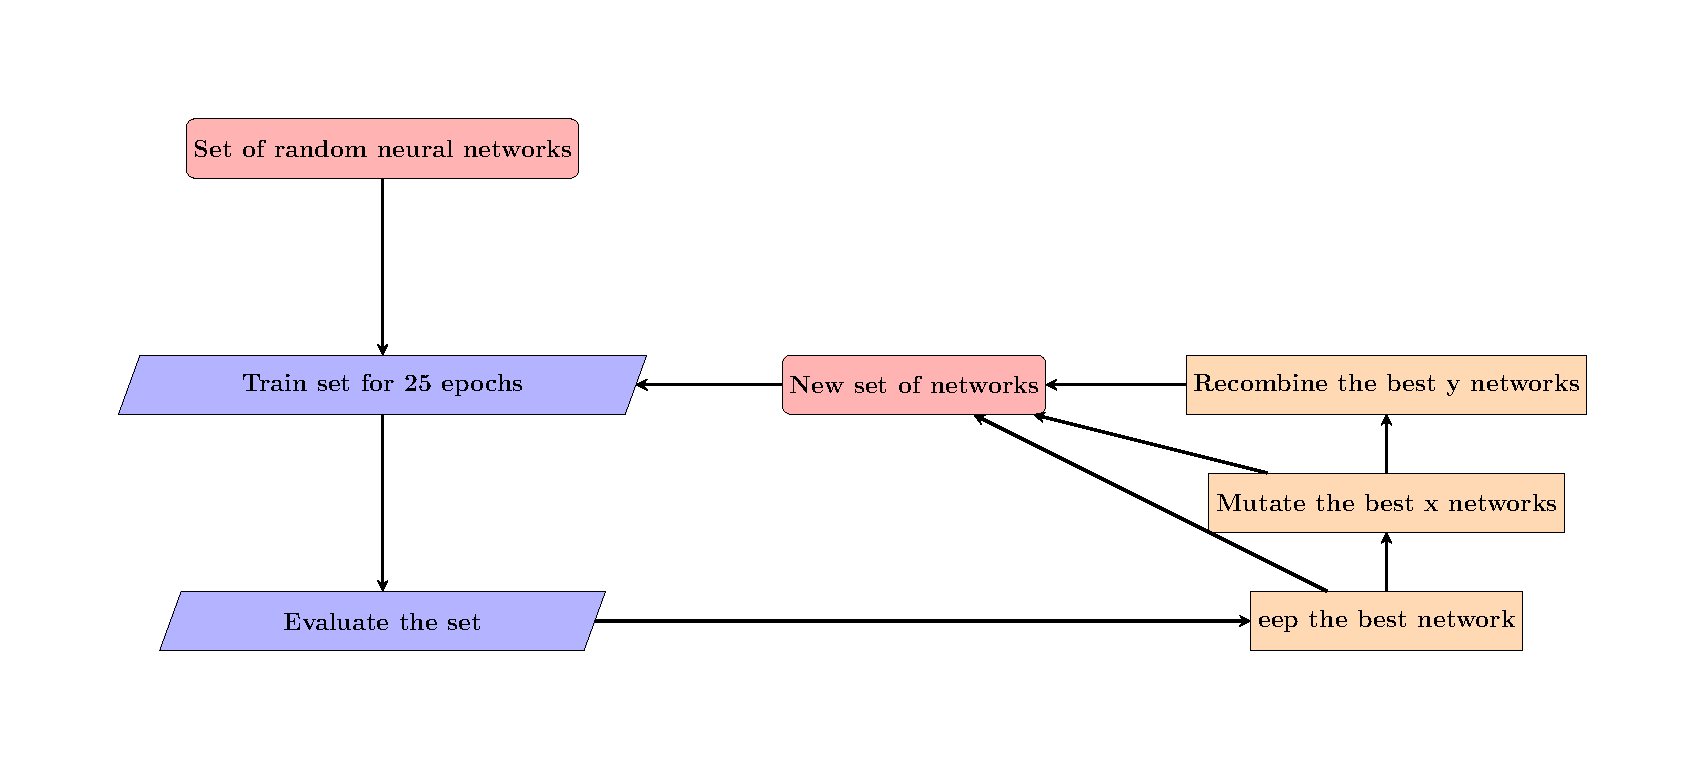
\includegraphics[width = \textwidth]{flowchart.pdf}
\end{frame}



\begin{frame}{Example of an evolutionary training}
    \begin{columns}
        \begin{column}{0.5\textwidth}
            \vspace{-0.4cm}
            \begin{itemize}
                \item Signal: \tHq
                \vspace{0.3cm}
                \item Background: \ttbar
                \vspace{0.3cm}
                \item Testing: nodes, layers, dropout
                \vspace{0.3cm}
                \item Fixed hyperparameters:
                    \begin{itemize}
                        \item Optimizer: Adam
                        \item Activation: relu, sigmoid
                        \item Batchsize: 1000
                        \item Epochs per generation: 25
                    \end{itemize}
            \end{itemize}
        \end{column}
            \begin{column}{0.5\textwidth}
                \begin{block}{Initial parameters}
                    \begin{itemize}
                        \item Layers: $1-10$
                        \item Nodes: $1-100$
                        \item Dropout: $0-1$
                    \end{itemize}
                \end{block}
                \begin{block}{Final parameters}
                    \begin{itemize}
                        \item Layers: $[2:6]$
                        \item Nodes: $[30:90]$
                        \item Dropout: $[0.1:0.7]$
                    \end{itemize}
                \end{block}
        \end{column}
    \end{columns}
\end{frame}


%\begin{frame}{ROC and Separation}
%    \begin{columns}
%        \begin{column}{0.5\textwidth}
%            \begin{figure}
%                \centering
%                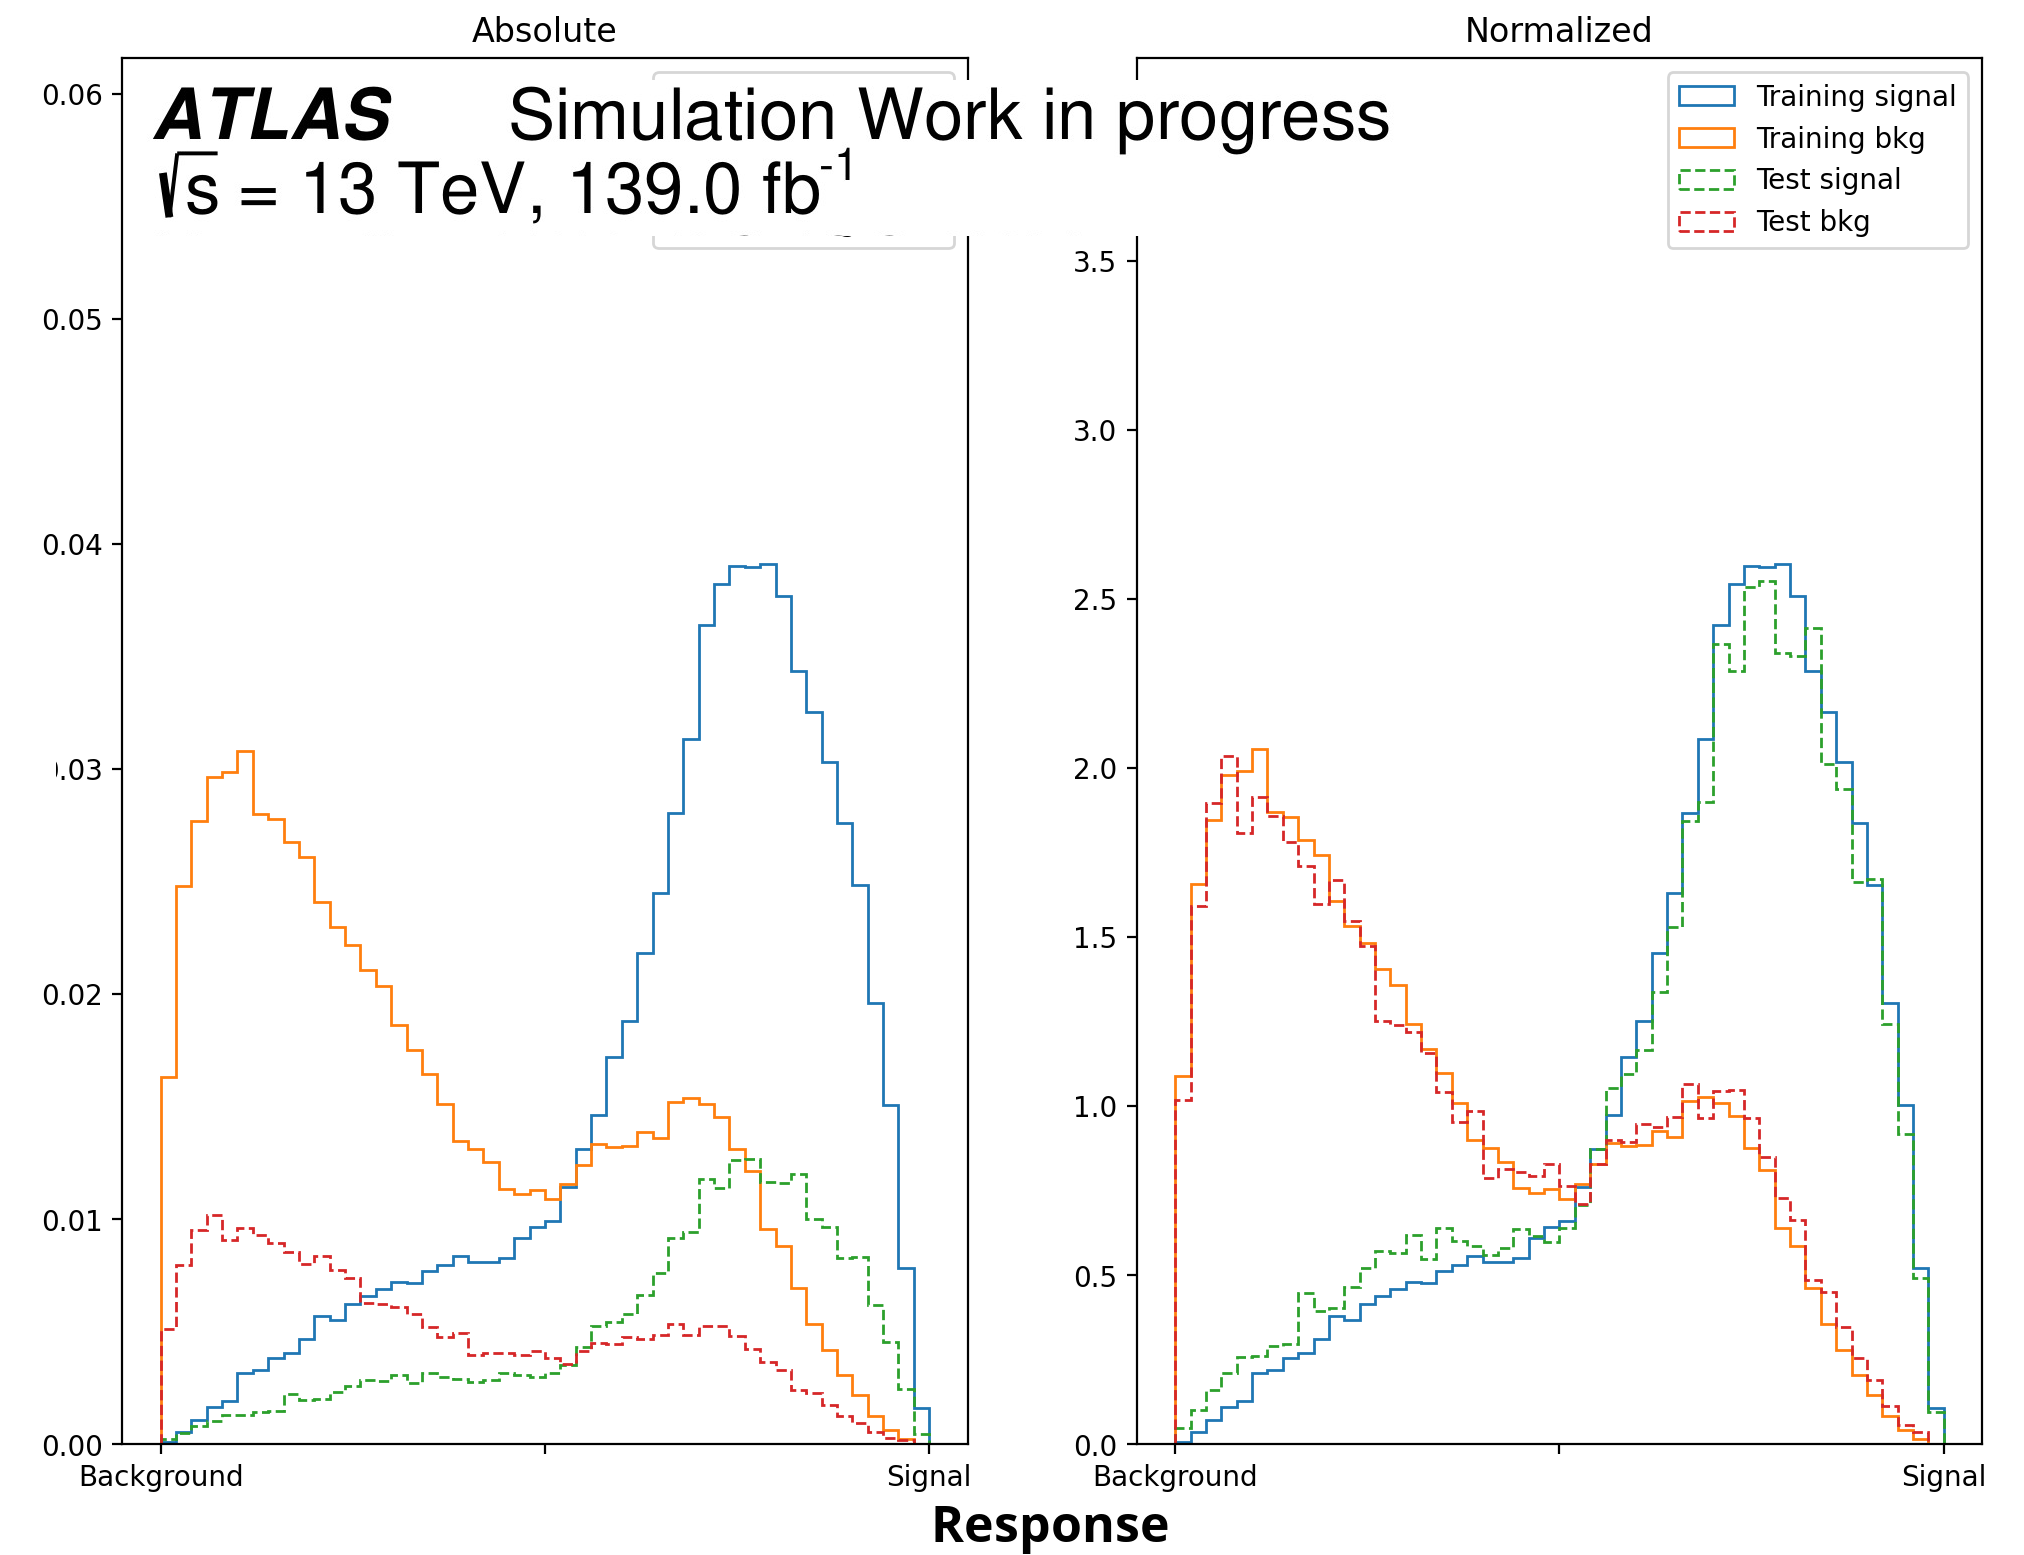
\includegraphics[width = \textwidth]{evo_response.png}
%            \end{figure}
%        \end{column}
%        \begin{column}{0.5\textwidth}
%            \begin{figure}
%                \centering
%                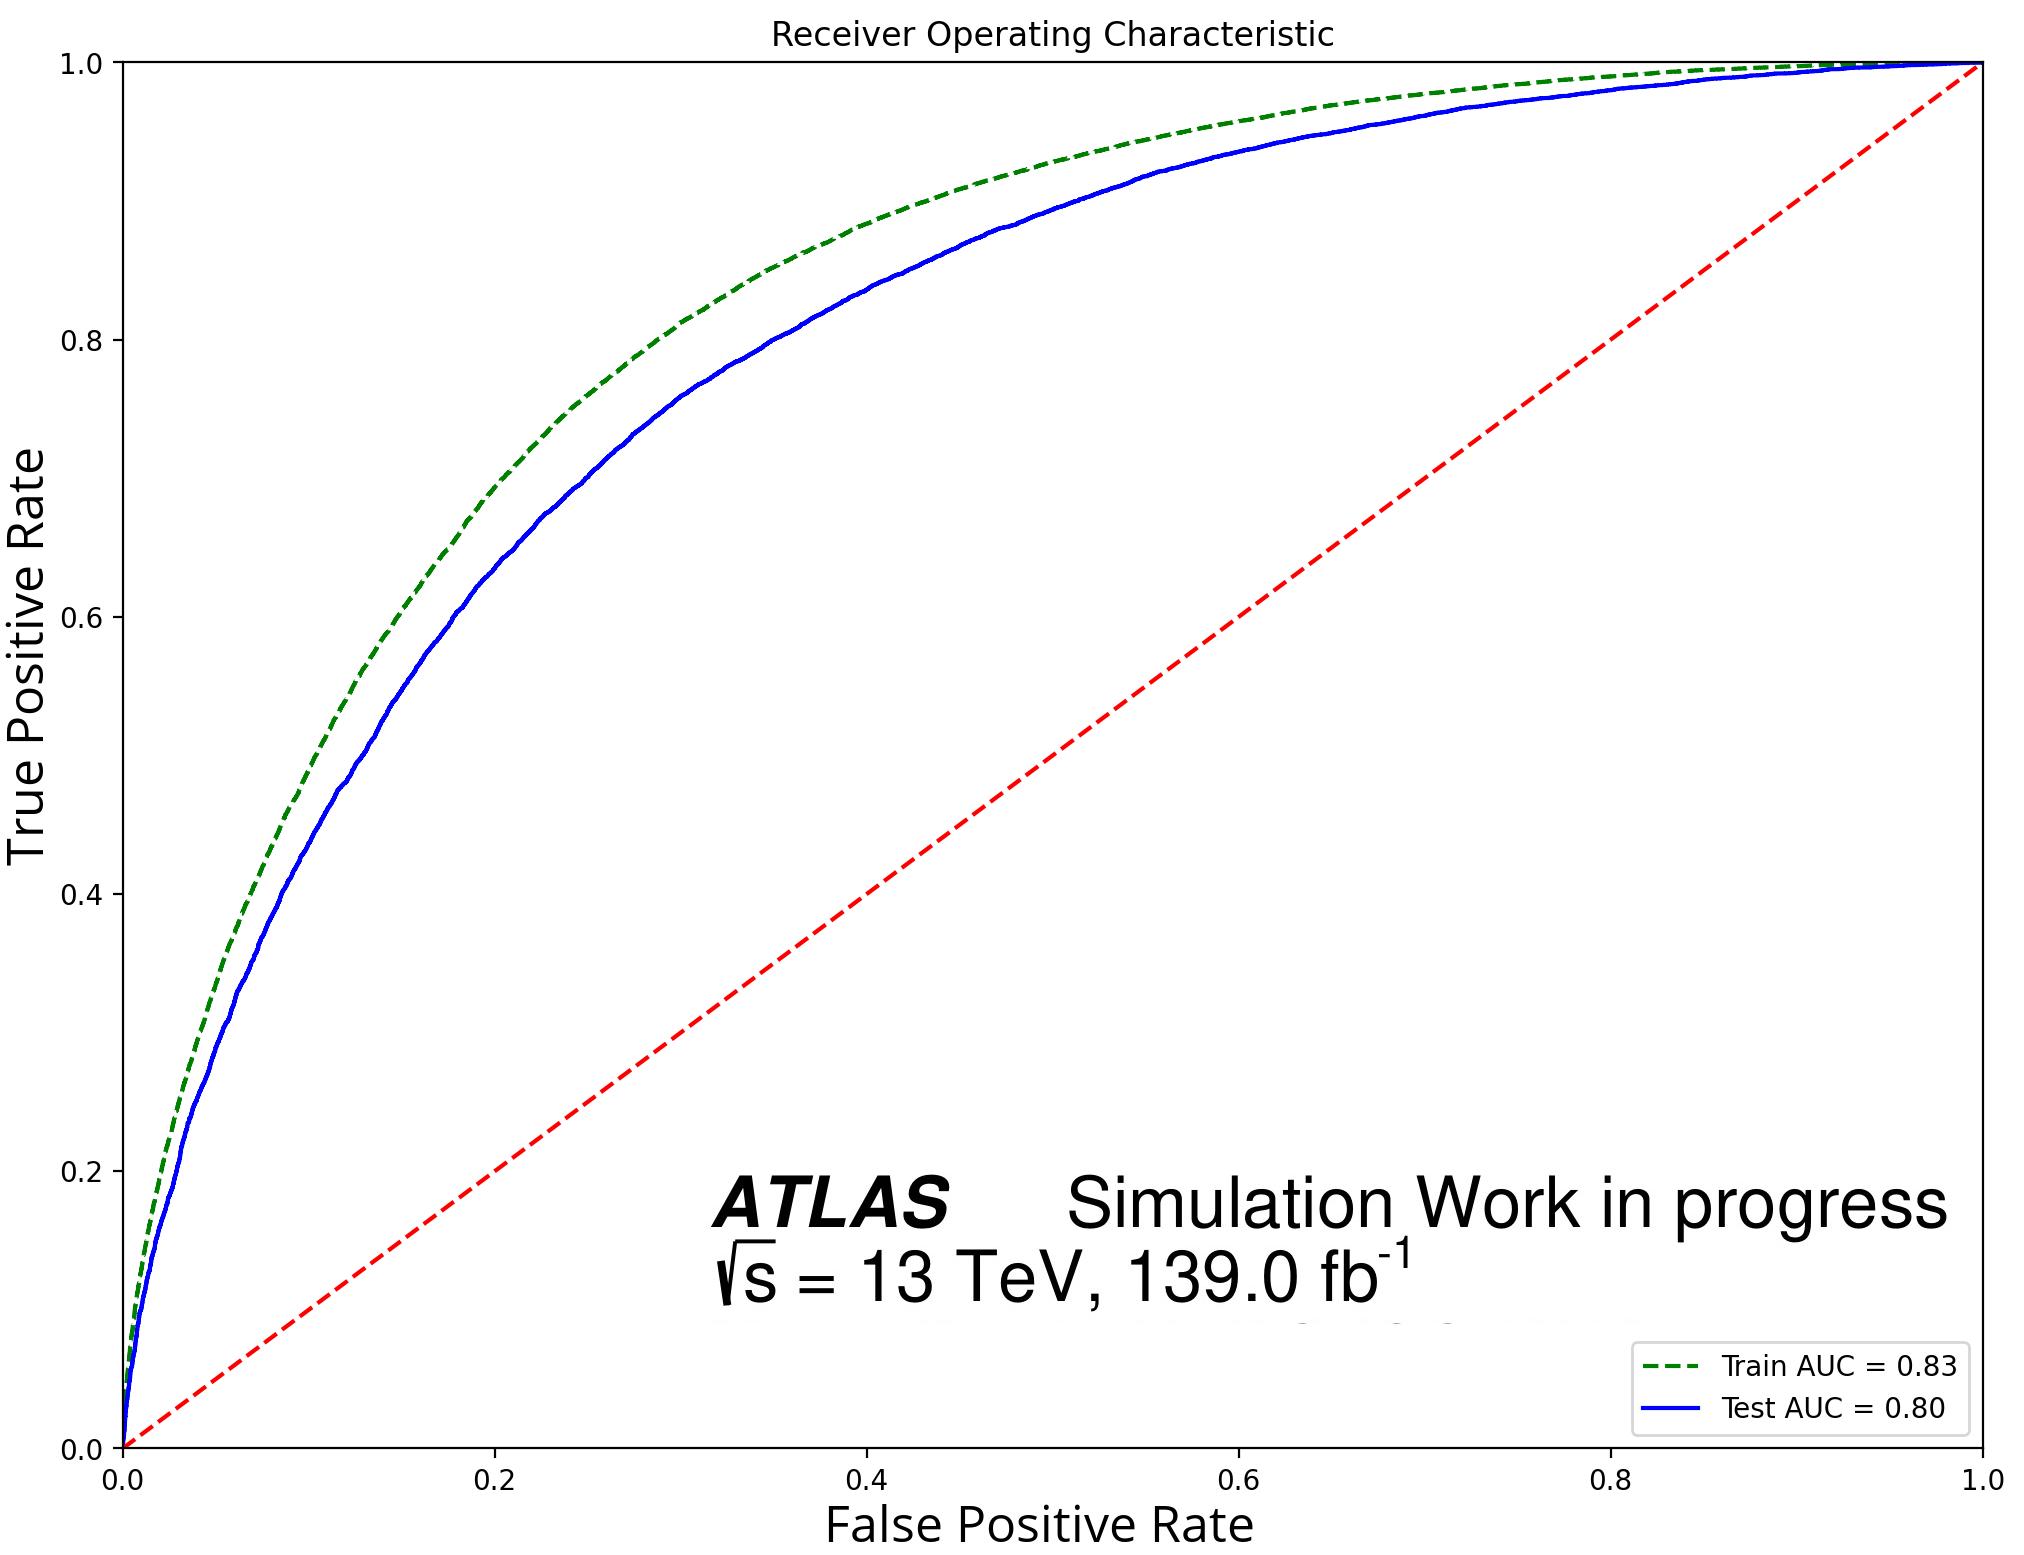
\includegraphics[width = \textwidth]{evo_ROC.png}
%            \end{figure}
%        \end{column}
%    \end{columns}
%\end{frame}

\begin{frame}{Comparing ROC to a grid search}
    \centering Computational ressources are comparable for both approaches. For the evolutionary optimisation a larger parameter space has been scanned.
    \begin{columns}
        \begin{column}{0.5\textwidth}
            \begin{figure}
                \centering
                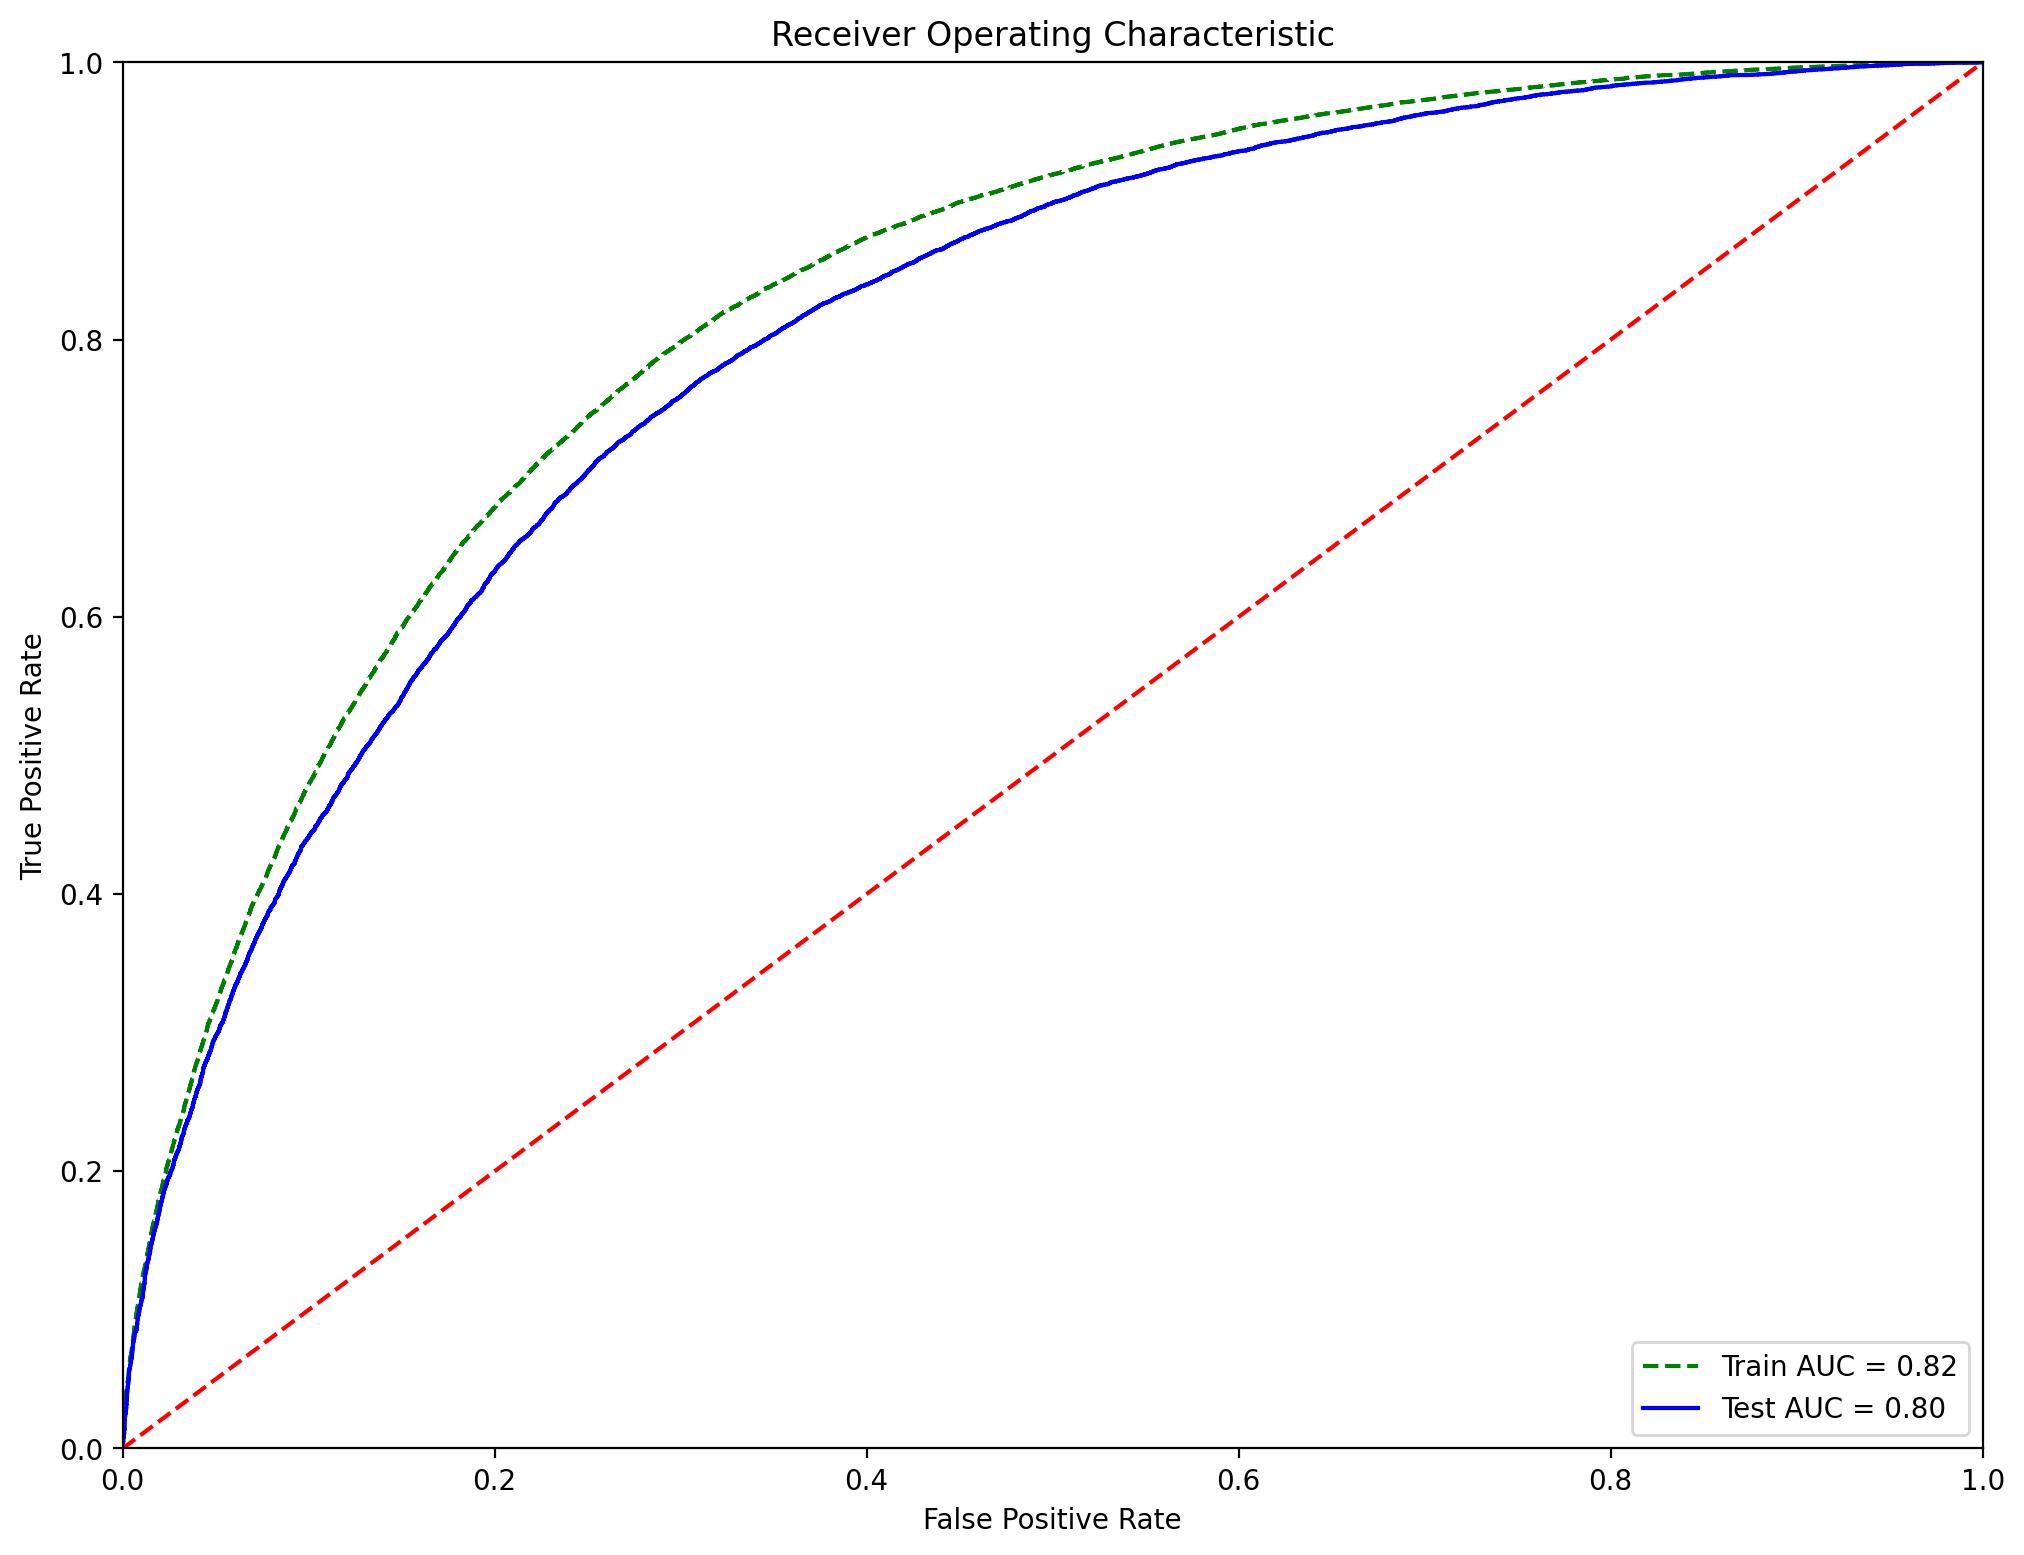
\includegraphics[width = \textwidth]{grid_ROC.png}
                \caption{Grid search}
            \end{figure}
        \end{column}
        \begin{column}{0.5\textwidth}
            \begin{figure}
                \centering
                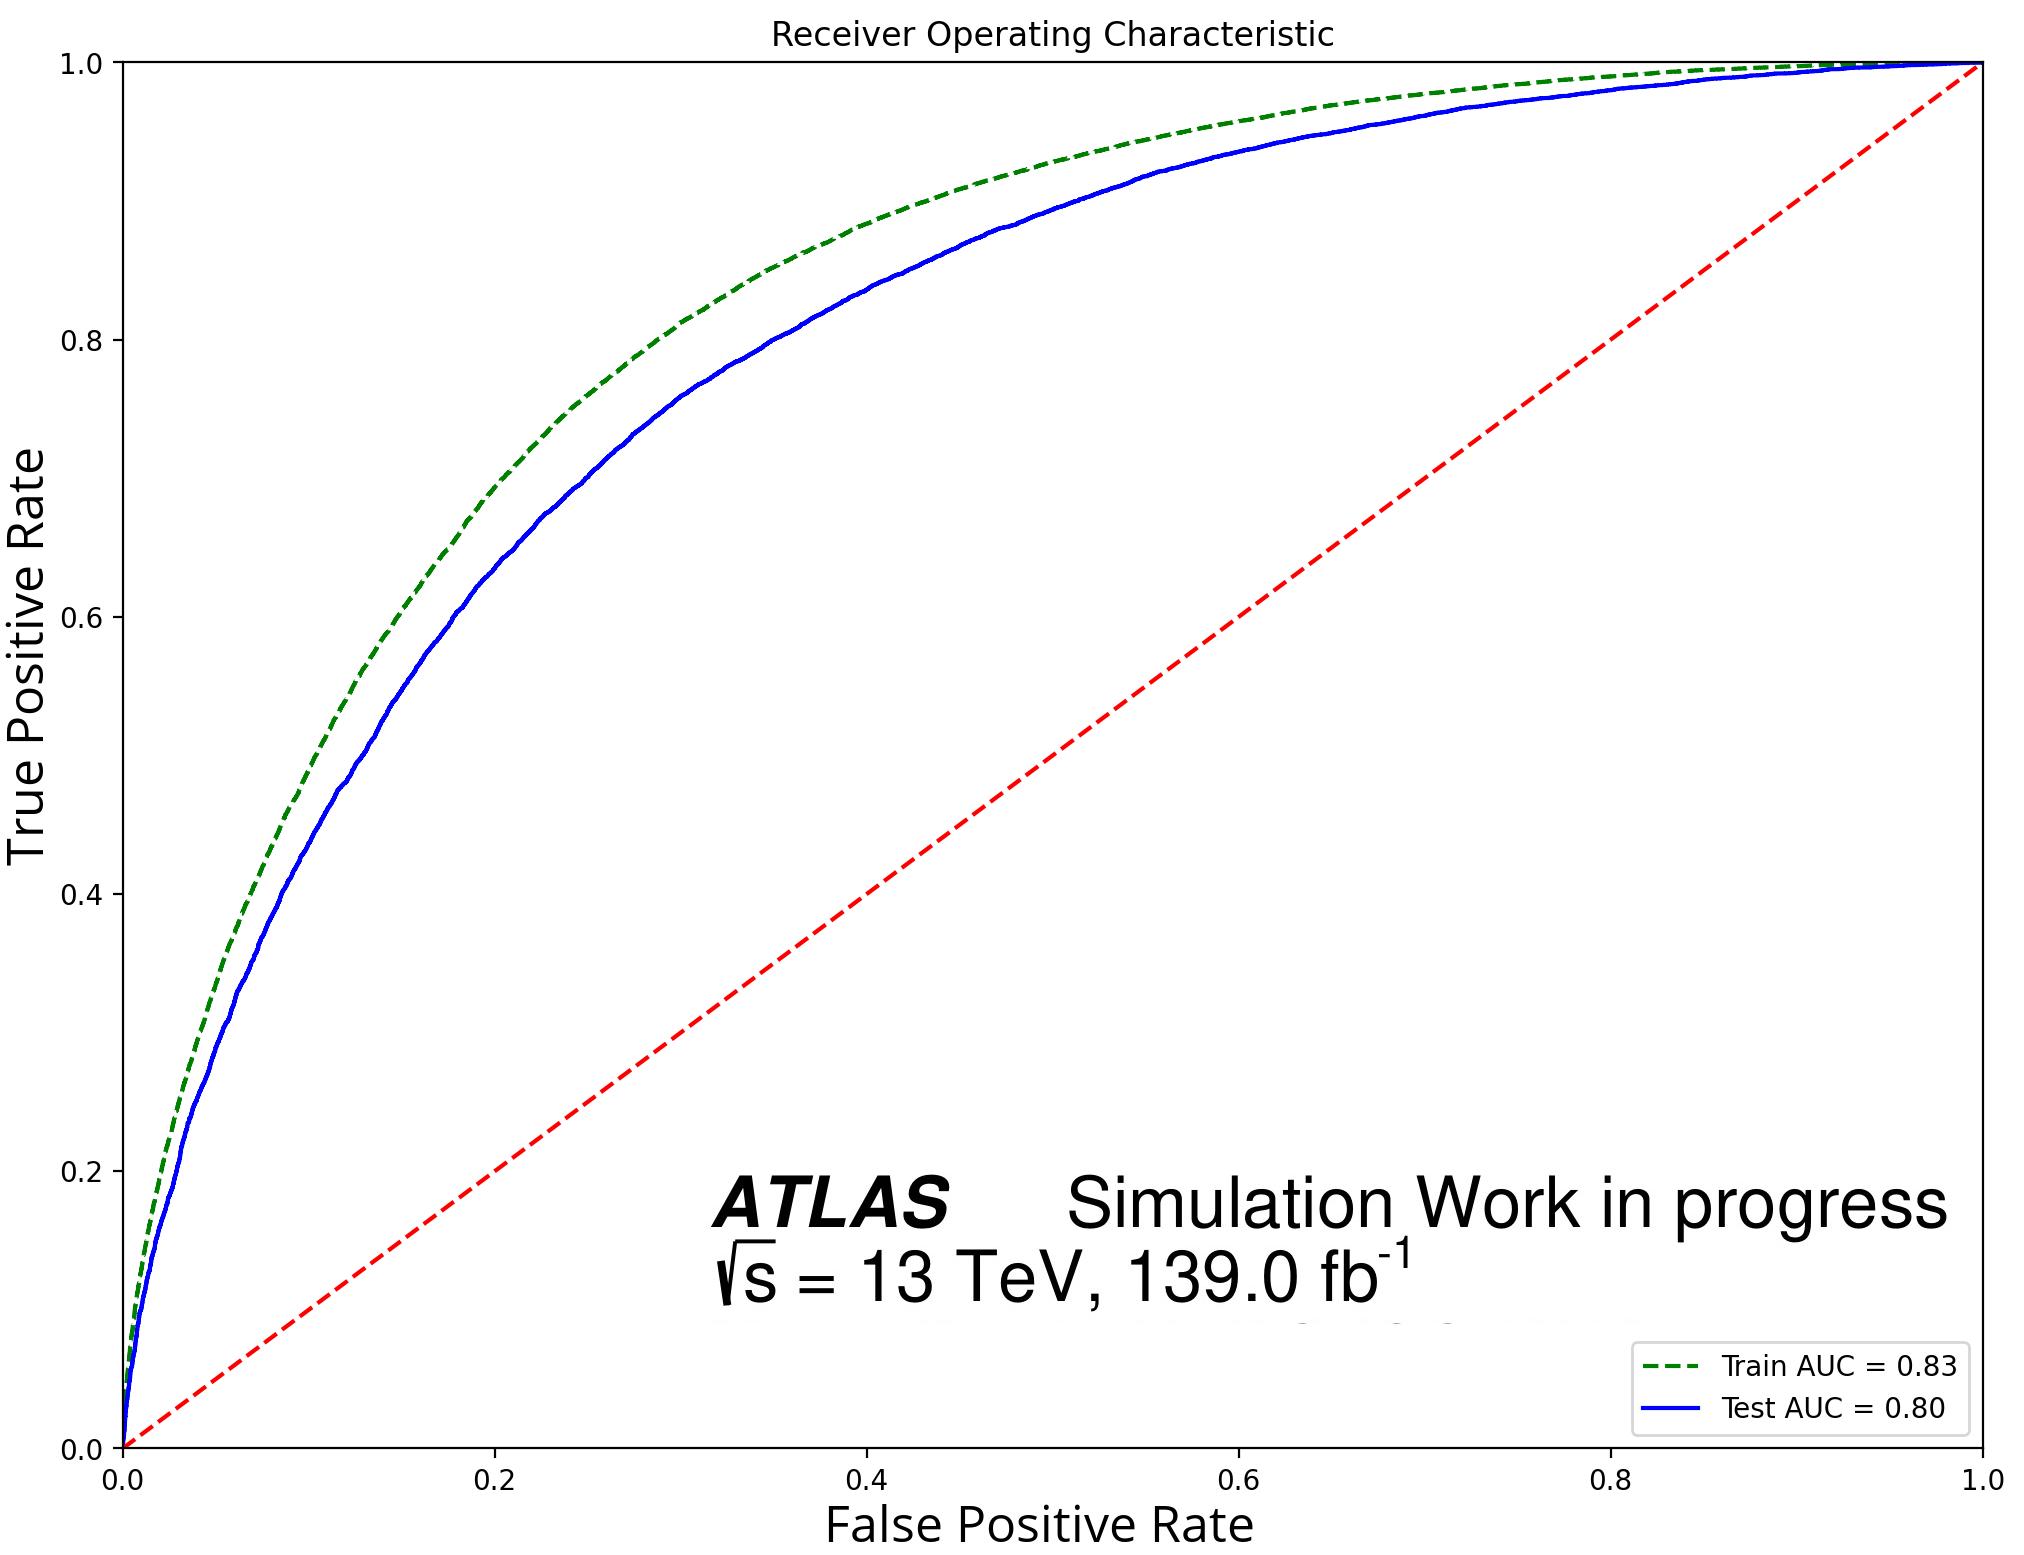
\includegraphics[width = \textwidth]{evo_ROC.png}
                \caption{Evolutionary search}
            \end{figure}
        \end{column}
    \end{columns}
\end{frame}


\begin{frame}{Comparing response to a grid search}
    \begin{columns}
        \begin{column}{0.5\textwidth}
            \begin{figure}
                \centering
                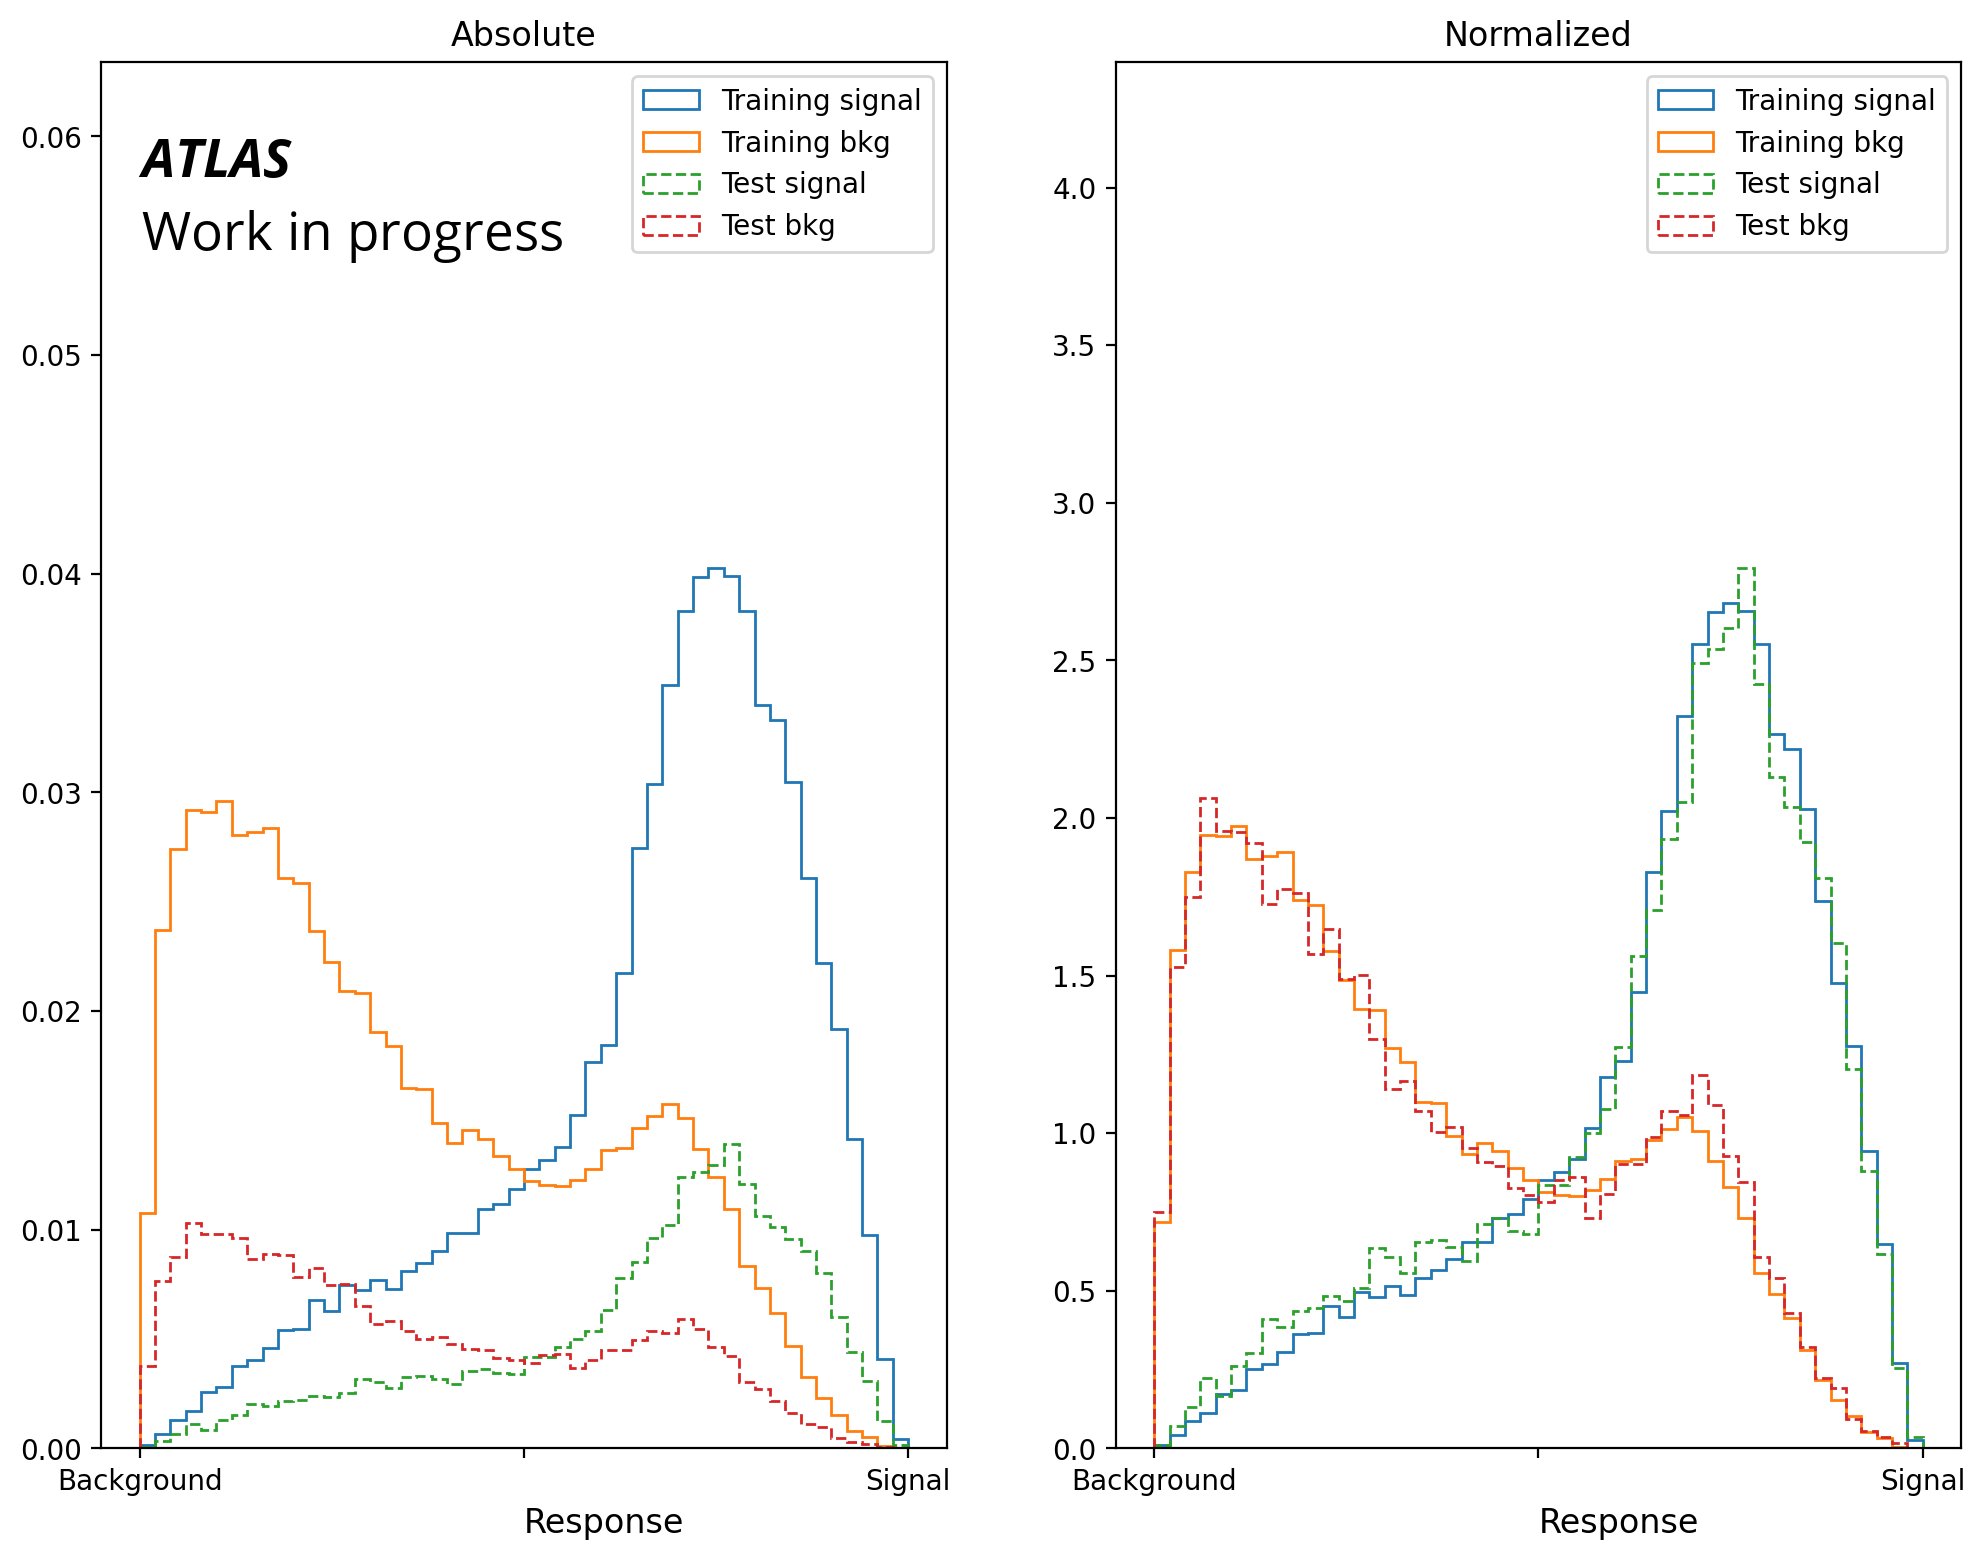
\includegraphics[width = \textwidth]{grid_response.png}
                \caption{Grid search}
            \end{figure}
        \end{column}
        \begin{column}{0.5\textwidth}
            \begin{figure}
                \centering
                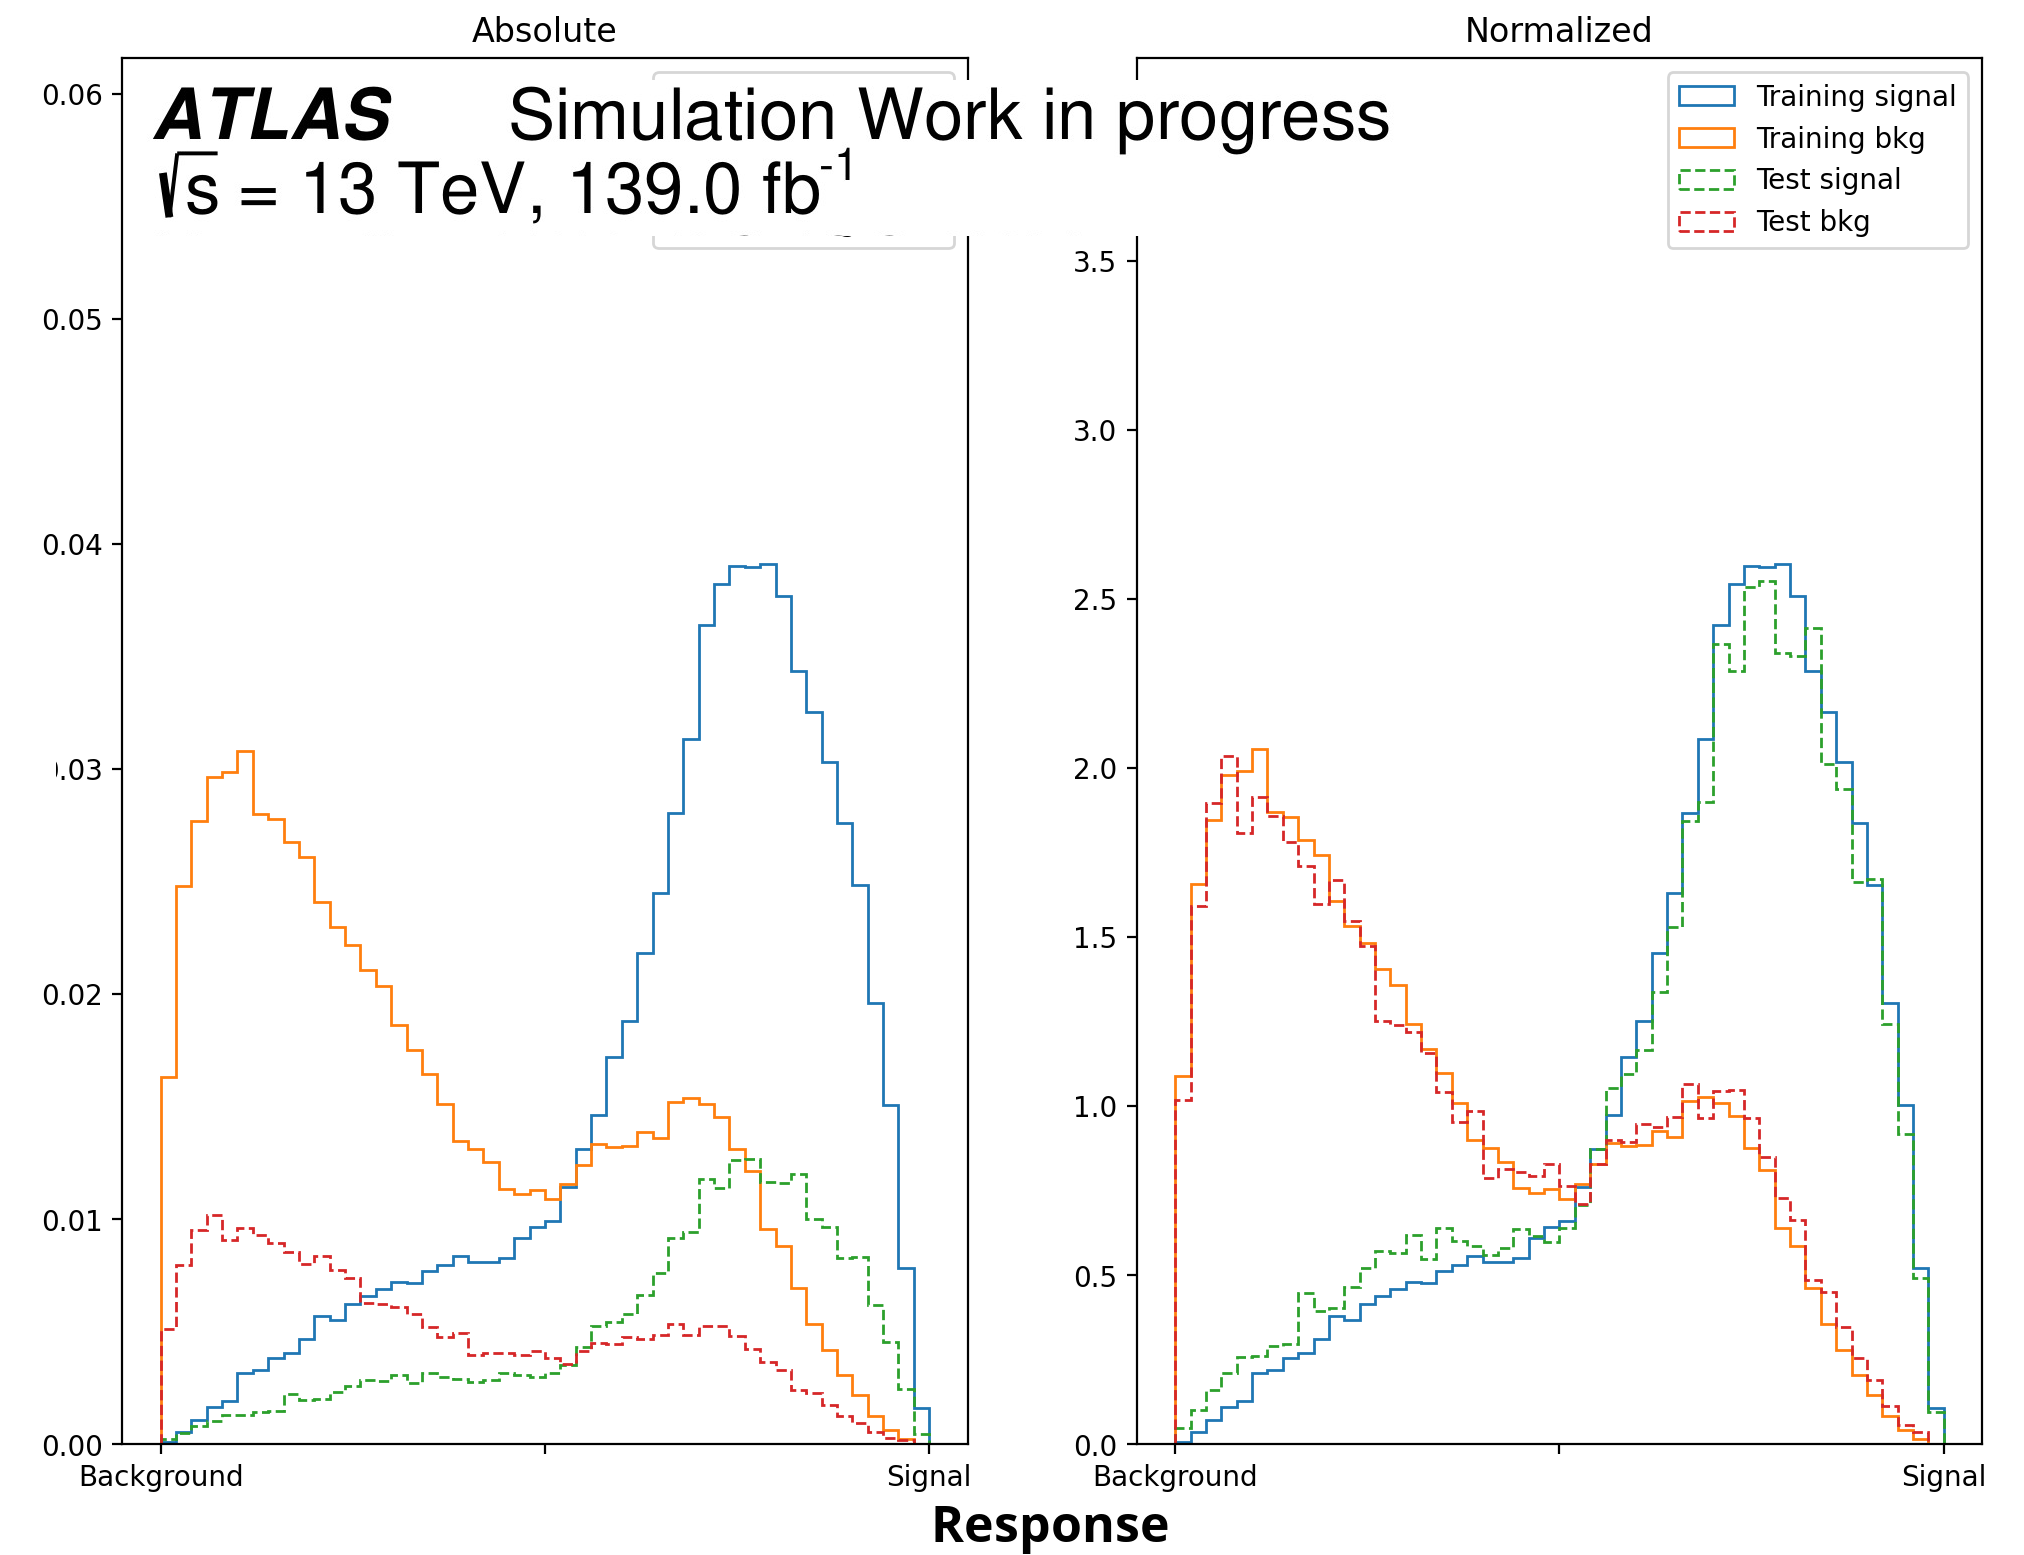
\includegraphics[width = \textwidth]{evo_response.png}
                \caption{Evolutionary search}
            \end{figure}
        \end{column}
    \end{columns}
\end{frame}